\documentclass{article}

\usepackage{Mathematics}
\pdftitle{IR-sensor-PDP2}

\title{\textbf{PDP2 \\ HSLU, Semester 4}}
\author{Matteo Frongillo}
\date{}

\begin{document}
\appendix
\renewcommand{\thesection}{I}
\part*{Appendix I}

\section{Distance-dependence of IR temperature detection}

\subsection{Data of the worst-case experiment}
The following worst-case temperature data are used:

\[
\begin{array}{c|c}
x\,[\mathrm{cm}] & T\,[^\circ\mathrm{C}]\\
\hline
5   & 50.00\\
10  & 45.00\\
20  & 41.50\\
30  & 36.50\\
40  & 29.75\\
50  & 27.00\\
60  & 26.00\\
70  & 24.75\\
80  & 24.25\\
90  & 24.00\\
100 & 24.00
\end{array}
\]

The ambient temperature is $T_{\mathrm{amb}}=23.5^\circ\mathrm{C}$.

\subsection{Regression exponential function}
The distance dependence is now modeled as an exponential function of the form

\[
T(x)=T_{\mathrm{amb}}+Ae^{Bx} \Longleftrightarrow T(x)-T_{\mathrm{amb}}=Ae^{Bx}.
\]

Linearizing the model gives

\[
\ln\!\bigl(T(x)-T_{\mathrm{amb}}\bigr)=\ln A+Bx.
\]

Defining

\[
Y_i=\ln\!\bigl(T_i-T_{\mathrm{amb}}\bigr),
\]

the regression becomes linear:

\[
Y_i=\alpha+Bx_i,
\qquad \text{with} \qquad \alpha=\ln A.
\]

The slope \(B\) is then given by

\[
B=\frac{\sum_i x_iY_i-\frac{1}{n}\left(\sum_i x_i\right)\left(\sum_i Y_i\right)}
{\sum_i x_i^2-\frac{1}{n}\left(\sum_i x_i\right)^2},
\]

and the intercept \(\alpha\) by

\[
\alpha=\bar{Y}-B\bar{x},
\]

where

\[
\bar{x}=\frac{\sum_i x_i}{n},
\qquad
\bar{Y}=\frac{\sum_i Y_i}{n}.
\]

\newpage
Finally,

\[
A=e^{\alpha}.
\]

Using the data in section 1.1, the fitted parameters are

\[
A=38.72,
\qquad
B=-0.04661,
\]

which gives

\[
T(x)=23.5+38.72e^{-0.04661x}.
\]

\subsection{Final step function}
To impose a conservative lower-bound behavior, the final model is defined piecewise as

\[
T(x)=
\begin{cases}
30, & \text{for } x\leq 38.28694,\\[6pt]
23.5+38.72e^{-0.04661x}, & \text{for } 38.28694<x<78.44575,\\[6pt]
24.5, & \text{for } x\geq 78.44575.
\end{cases}
\]

The first transition point was chosen such that

\[
23.5+38.72e^{-0.04661x}=30
\]

at

\[
x=38.28694\,\mathrm{cm},
\]

and the second transition point such that

\[
23.5+38.72e^{-0.04661x}=24.5
\]

at

\[
x=78.44575\,\mathrm{cm}.
\]

Thus, the piecewise function is continuous at both transition points.

\subsection{Graphic}
\begin{center}
    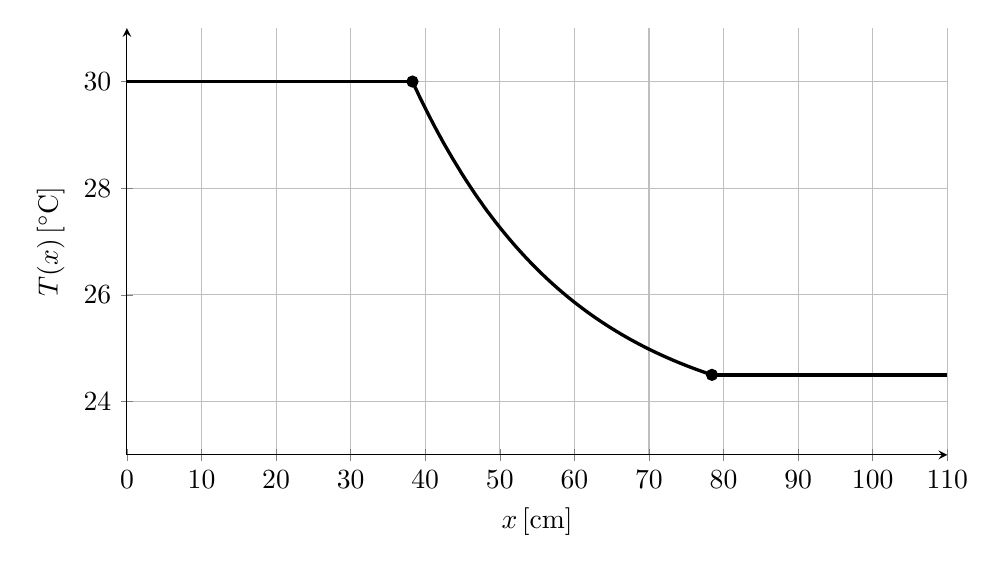
\begin{tikzpicture}
        \begin{axis}[
            width=12cm,
            height=7cm,
            xlabel={$x\,[\mathrm{cm}]$},
            ylabel={$T(x)\,[^\circ\mathrm{C}]$},
            xmin=0, xmax=110,
            ymin=23, ymax=31,
            domain=0:110,
            samples=200,
            axis lines=left,
            grid=both
        ]
    
        % First branch: T(x)=30 for x <= 38.28694
        \addplot[
            very thick,
            domain=0:38.28694
        ] {30};
    
        % Second branch: T(x)=23.5+38.72 e^{-0.04661x} for 38.28694 < x < 78.44575
        \addplot[
            very thick,
            domain=38.28694:78.44575
        ] {23.5 + 38.72*exp(-0.04661*x)};
    
        % Third branch: T(x)=24.5 for x >= 78.44575
        \addplot[
            very thick,
            domain=78.44575:110
        ] {24.5};
    
        % Closed points
        \addplot[only marks, mark=*, mark size=2pt]
        coordinates {
            (38.28694,30)
            (78.44575,24.5)
        };
    
        \end{axis}
    \end{tikzpicture}
\end{center}

\end{document}
